\documentclass{subfiles}
\begin{document}
Occupandocisi di analisi di immagini digitali, capita spesso di aver a che fare con immagini soggette a rumore di varia natura.
Risulta dunque necessario poter ottenere un immagine quanto più possibile priva di rumore.
Passando a discutere come porre rimedio a tale problema
\begin{wrapfigure}{r}{0.425\textwidth}
    \centering
    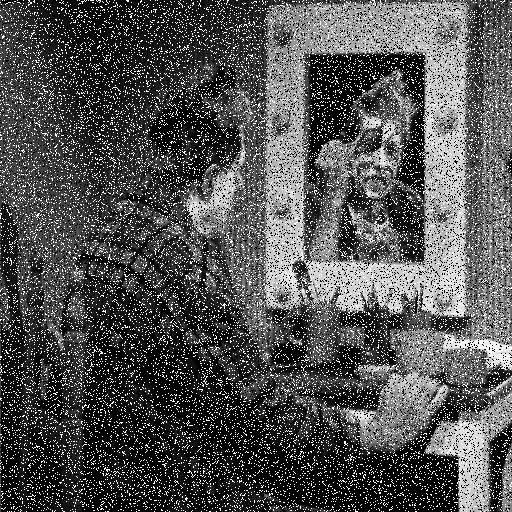
\includegraphics[scale = 0.325]{../Images/Clown/NoisyClown.png}
    \caption{Clown soggetto a rumore.}
    \label{fig:4.4}
\end{wrapfigure}
si consideri \emph{Figura \ref{fig:4.4}}.
Questa è un'immagine soggetta a rumore ``sale e pepe'', così definito perché aggiunge pixel bianchi e neri sparsi quà e là per l'immagine.

Considerando uno dei metodi utilizzati per rimuovere il rumore, si analizza il filtro mediano.
Questi è un filtro non convolutivo, che segue una logica molto semplice.  Si considera una finestra \(W\) e la si fa scorrere sull'immagine,
secondo logica raster, i pixel della finestra sono ordinati per tonalità di colore, e similarmente quel che si fa con un filtro convolutivo,
si seleziona il pixel centrale di \(W\) e si sostituisce a questi, quello che nella sequenza dei pixel ordinati risulta essere in posizione centrale.

\begin{Remark*}
    il filtro mediano non è perfetto. Questi presenta alcune problematiche, più o meno evidenti a seconda delle dimensioni della finestra.
    Principali problemi risultano essere quello ai bordi, e il fatto che all'aumentare delle dimensioni della finestra, l'immagine tende a sfocare,
    finendo col
    \begin{wrapfigure}{l}{0.425\textwidth}
        \centering
        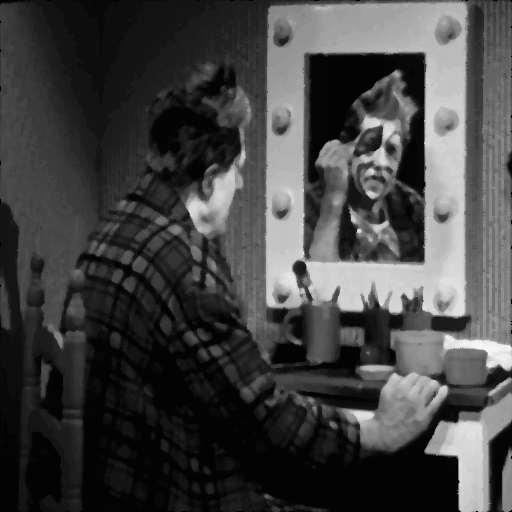
\includegraphics[scale = 0.325]{../Images/Clown/MedianFilteredClown.png}
        \caption{Filtro mediano applicato a \emph{Figura \ref{fig:4.4}}.}
        \label{fig:4.5}
    \end{wrapfigure}
    somigliare ad un filtro di media. Infine, del rumore potrebbe non essere eliminato, se la finestra è troppo piccola
\end{Remark*}

Analizzando dunque il caso di \emph{Figura \ref{fig:4.4}}, applicando un'opportuna implementazione dell'algoritmo sopra citato,
nel codice a seguire è fornito dall'istruzione \lstinline[language = MATLAB]{medfilt}, si ottiene quanto in \emph{Figura \ref{fig:4.5}}.
\begin{center}
    \begin{lstlisting}[language = MATLAB]
        % caricamento dell'immagine con rumore
        denoisedClown = medfil2(NoisyClown);
        figure; imshow(denoisedClown, [0, 255]);        
    \end{lstlisting}
\end{center}

Nel caso di rumore persistente, si può provare ad adottare una o più delle seguenti tecniche.
\begin{enumerate}
    \item Si procede con l'applicare nuovamente il filtro, aumentando opportunamente le dimensioni della finestra.
          Banalmente se si applicasse con le stesse dimensioni, verosimilmente l'immagine risulterebbe immutata.

    \item Limitandosi unicamente ai pixel soggetti a rumore, si applica nuovamente il filtro.
          Utile nel caso di finestre sufficientemente grandi.
\end{enumerate}


% Volendo provare a migliorare ulteriormente l'immagine, alcune soluzioni sono le seguenti:
% \begin{itemize}
%     \item si applica nuovamente il filtro, cambiando le dimensioni della finestra.
%           Questo però risulta oneroso, proprio perché si deve rieseguire l'intero filtraggio;
%     \item si riapplica il filtro, concentrandosi unicamente sui pixel soggetti a rumore.
%           Risulta poco utile se la finestra ha dimensioni molto piccole.
% \end{itemize}

% \footnotetext[5]{Nel caso di \emph{Figura \ref{fig:4.4}} questa è soggetta a rumore "sale e pepe". Si noti che esistono però altri tipi di rumore.}
\end{document}